\documentclass[11pt]{article}
\usepackage{report-style}
\begin{document}
\hypersetup{pageanchor=false}

\begin{titlepage}
  \centering
  \vspace*{0.5in}
  \gbmlogo\par
  \vspace{0.5in}
  {\LARGE\bfseries GBM Cloud\par}
  \vspace{0.18in}
  {\Large\bfseries Project 5 Technical Report\par}
  \vspace{0.22in}
  {\large\itshape Design and Deployment of a Secure Cloud Website\par}
  \vspace{0.08in}
  {\normalsize\itshape A Custom Multi-Agent AI System\par}
  \vfill
  \begin{minipage}{0.78\textwidth}
    \textbf{Name:} Sai Abhinav Vurakaranam\\[7pt]
    \textbf{Course:} CSCE 412\\[7pt]
    \textbf{Institution:} Texas A\&M University\\[7pt]
    \textbf{Date:} November 8, 2026\\[14pt]
    \textbf{Website:} \url{https://csce412abhivur.me/}\\[7pt]
    \textbf{Private repository:}\\
    \url{https://github.com/abhivur/CSCE412-Project5}
  \end{minipage}
  \vspace*{0.6in}
\end{titlepage}

\pagenumbering{roman}
\hypersetup{pageanchor=true}
\tableofcontents
\clearpage
\pagenumbering{arabic}

\section{Project Overview and Website Design}
\subsection{Purpose and scope}
GBM Cloud combines a public cloud-learning website with an executable system of specialized artificial intelligence (AI) agents. The website provides an approachable introduction to secure static hosting. The engineering system plans work, builds content, deploys approved Amazon Web Services (AWS) configurations, verifies actual behavior, and diagnoses a reversible infrastructure failure.

This report addresses the technical reviewer for CSCE 412 Project 5. It explains the implemented system, the deployment procedure, the security controls, and the evidence supporting recovery. The deployed website is \url{https://csce412abhivur.me/}. Source code is associated with the private repository \url{https://github.com/abhivur/CSCE412-Project5}; a reviewer needs repository access to view private content.

\subsection{Website structure and interaction}
Five main pages share consistent navigation, typography, spacing, and responsive styling:
\begin{itemize}
  \item \textbf{Home, \filepath{index.html}:} Introduces GBM Cloud and the secure delivery architecture, with links to solutions and the launch planner.
  \item \textbf{Solutions, \filepath{solutions.html}:} Presents six educational cloud blueprints. Category and difficulty filters combine to narrow the visible cards.
  \item \textbf{Resources, \filepath{resources.html}:} Explains architecture, prelaunch verification, and private-origin security through three learning articles.
  \item \textbf{About, \filepath{about.html}:} Describes the student project, its purpose, and its Texas A\&M-inspired identity.
  \item \textbf{Launch planner, \filepath{planner.html}:} Generates a checklist from a project name, launch scope, and focus area.
\end{itemize}
The planner is the principal client-side JavaScript feature. Visitors create a checklist, mark completed tasks, view progress, and download the current checklist as a text file. Browser \texttt{localStorage} preserves the plan between visits. Reset removes the saved plan and the selected-solution query parameter. If storage is unavailable, the planner remains usable in memory. This feature creates local guidance, rather than provisioning cloud resources for visitors.

A custom \filepath{404.html} handles missing resources. Three older page addresses remain available as compatibility pages with current branding. The static checker therefore evaluates nine HTML files: five main pages, three compatibility pages, and the error page. The published build contains 16 files, including six shared assets and the robots file.

\subsection{Visual design and validation scope}
The design uses white backgrounds, muted maroon accents, neutral tones, and locally stored cloud illustrations. Shared CSS and JavaScript support mobile navigation and flexible layouts. The cloud logo represents the current GBM Cloud identity; the project is a student implementation and does not claim official university affiliation.

Recorded local checks passed for navigation, references, assets, and page structure. The current automated suite passed 56 Python tests and 12 JavaScript tests. JavaScript tests cover filtering, checklist persistence, reset, downloads, unavailable storage, and mobile-menu events. These checks exercise program behavior; they do not establish visual correctness on every physical device. A browser harness is also provided in \filepath{tests/browser.html}.

\section{AWS Infrastructure Architecture}
\subsection{Services and delivery path}
Figure~\ref{fig:aws} separates website traffic from DNS resolution and certificate configuration. The deployment uses Amazon Simple Storage Service (S3), Amazon CloudFront, Amazon Route 53, and AWS Certificate Manager (ACM). It does not require a continuously running backend, virtual machine, or database.

\begin{figure}[htbp]
\centering
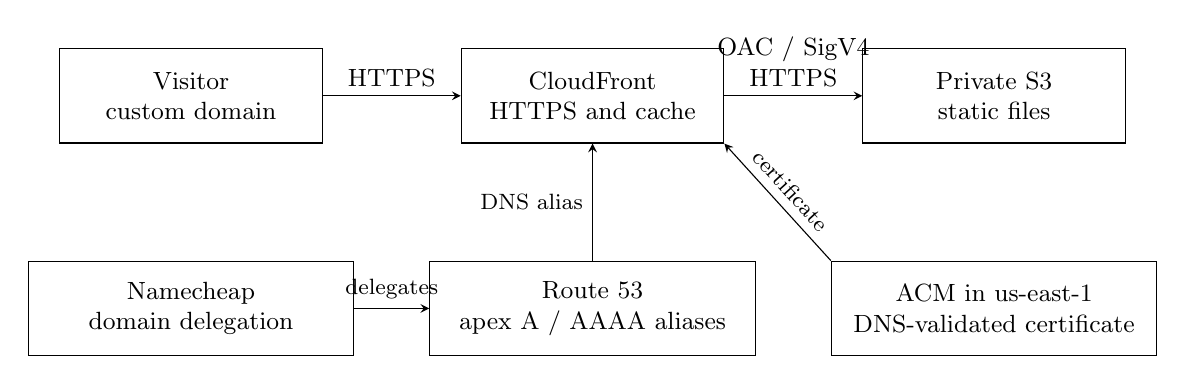
\begin{tikzpicture}[font=\small,>=stealth,
  box/.style={draw,align=center,minimum height=12mm,text width=31mm},
  support/.style={draw,align=center,minimum height=12mm,text width=39mm}]
  \node[box] (visitor) at (0,0) {Visitor\\custom domain};
  \node[box] (cf) at (5.1,0) {CloudFront\\HTTPS and cache};
  \node[box] (s3) at (10.2,0) {Private S3\\static files};
  \draw[->] (visitor) -- node[above]{HTTPS} (cf);
  \draw[->] (cf) -- node[above,align=center]{OAC / SigV4\\HTTPS} (s3);
  \node[support] (domain) at (0,-2.7) {Namecheap\\domain delegation};
  \node[support] (dns) at (5.1,-2.7) {Route 53\\apex A / AAAA aliases};
  \node[support] (acm) at (10.2,-2.7) {ACM in us-east-1\\DNS-validated certificate};
  \draw[->] (domain) -- node[above,font=\footnotesize]{delegates} (dns);
  \draw[->] (dns) -- node[left,font=\footnotesize]{DNS alias} (cf);
  \draw[->] (acm.north west) -- node[above,sloped,font=\footnotesize]{certificate} (cf.south east);
\end{tikzpicture}
\caption{AWS architecture. Website content follows the upper path. The lower path provides domain delegation, DNS resolution, and certificate configuration.}
\label{fig:aws}
\end{figure}

\begin{itemize}
  \item \textbf{S3:} Stores website files in \texttt{us-east-1}. The bucket is \filepath{csce412abhivur-me-project5}. It uses the S3 REST endpoint as its origin, with public access blocked.
  \item \textbf{CloudFront:} Distribution \texttt{E1YB5Q5M7QMQA9} caches and delivers content, redirects HTTP requests to HTTPS, and uses \texttt{index.html} as the default root object. Its AWS hostname is \url{https://d110ckj7cjf58d.cloudfront.net/}.
  \item \textbf{ACM:} Supplies the DNS-validated certificate for \texttt{csce412abhivur.me}. The certificate is in \texttt{us-east-1}, as required for CloudFront viewer certificates~\cite{acm}.
  \item \textbf{Route 53:} Hosts the public DNS zone. Apex A and AAAA alias records point the domain to CloudFront. A validation CNAME establishes certificate ownership.
  \item \textbf{Namecheap:} Registers the custom domain. Its nameserver delegation points to the four authoritative nameservers assigned by Route 53.
\end{itemize}

\subsection{Content publication and errors}
The deterministic site builder writes the static build to \filepath{dist/}. Publication uploads the generated files to S3, records their SHA-256 hashes, and requests a CloudFront invalidation. Later verification compares fetched page and asset content with the recorded publication manifest. Uploads do not automatically delete remote objects.

CloudFront retrieves origin files through Origin Access Control (OAC). OAC uses AWS Signature Version 4 (SigV4) and always signs origin requests. The bucket permits object reads from the designated CloudFront distribution. This preserves a public website while keeping direct S3 access private~\cite{oac}.

CloudFront maps origin 403 and 404 responses to \filepath{/404.html}, retaining an HTTP 404 response and an error-cache time to live of zero. Mapping 403 is necessary because a private S3 origin can return Access Denied for a missing key. Returning a real 404 avoids disguising missing resources as successful page loads.

\section{AI Agent Architecture}
\subsection{Specialized roles}
The implementation uses five specialized agents, exceeding the minimum of four. These are distinct role configurations in a custom Python orchestrator, rather than five continuously running services.
\begin{itemize}
  \item \textbf{Planner:} Inspects the project, interprets requirements, and returns tasks for the website, infrastructure, and verification roles. It cannot deploy infrastructure.
  \item \textbf{Website:} Inspects content, edits bounded page introductions, renders the site, and checks local links and assets. Its tools operate on the website implementation.
  \item \textbf{Infrastructure:} Inspects actual resources, prepares a stage-specific change plan, and requests approval to apply the exact plan. In local mode it produces an architecture specification instead of claiming deployment.
  \item \textbf{Verification:} Executes local or live checks. Live checks measure DNS, TLS, redirects, page and asset responses, origin restrictions, CloudFront configuration, and OAC signing. It can also collect DNS diagnostics.
  \item \textbf{Diagnosis:} Reviews failed verification, inspects infrastructure, explains the likely cause, prepares recorded recovery, and requests human approval when restoration is authorized.
\end{itemize}

Figure~\ref{fig:agents} shows the communication path. The orchestrator passes structured messages and upstream results between roles. A failed live report can trigger diagnosis; recovery still requires a separate passing verification result.

\begin{figure}[htbp]
\centering
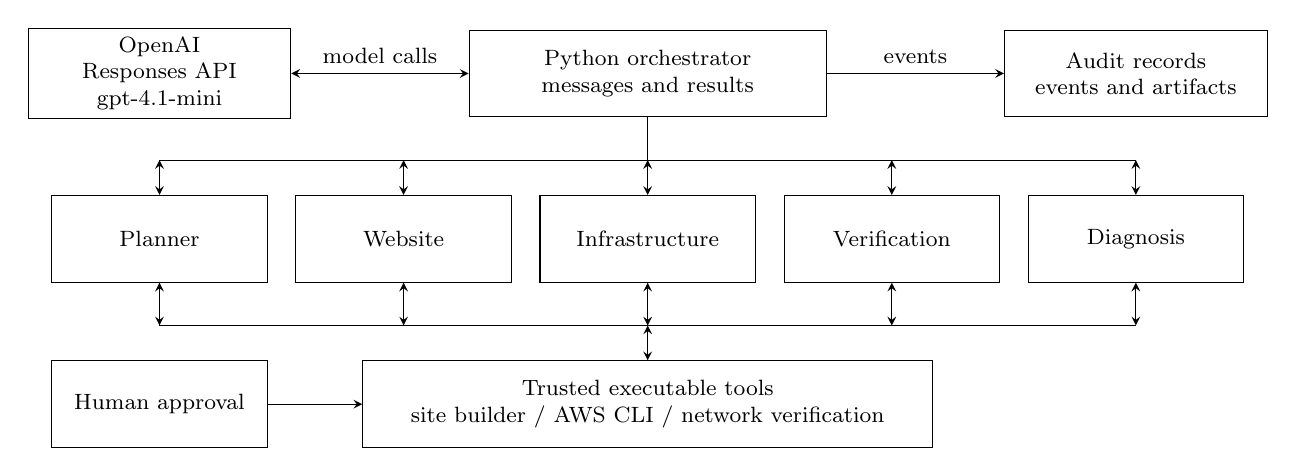
\begin{tikzpicture}[font=\footnotesize,>=stealth,
  box/.style={draw,align=center,text width=25mm,minimum height=11mm}]
  \node[box,text width=31mm] (model) at (0,0) {OpenAI\\Responses API\\gpt-4.1-mini};
  \node[box,text width=43mm] (orch) at (6.2,0) {Python orchestrator\\messages and results};
  \node[box,text width=31mm] (audit) at (12.4,0) {Audit records\\events and artifacts};
  \draw[<->] (model) -- node[above]{model calls} (orch);
  \draw[->] (orch) -- node[above]{events} (audit);
  \node[box] (planner) at (0,-2.1) {Planner};
  \node[box] (web) at (3.1,-2.1) {Website};
  \node[box] (infra) at (6.2,-2.1) {Infrastructure};
  \node[box] (verify) at (9.3,-2.1) {Verification};
  \node[box] (diag) at (12.4,-2.1) {Diagnosis};
  \draw (orch.south) -- (6.2,-1.1);
  \draw (0,-1.1) -- (12.4,-1.1);
  \foreach \role in {planner,web,infra,verify,diag} {
    \draw[<->] (\role.north |- 0,-1.1) -- (\role.north);
  }
  \node[box,text width=70mm] (tools) at (6.2,-4.2) {Trusted executable tools\\site builder / AWS CLI / network verification};
  \node[box] (human) at (0,-4.2) {Human approval};
  \draw (0,-3.2) -- (12.4,-3.2);
  \foreach \role in {planner,web,infra,verify,diag} {
    \draw[<->] (\role.south) -- (\role.south |- 0,-3.2);
  }
  \draw[<->] (6.2,-3.2) -- (tools.north);
  \draw[->] (human) -- (tools);
\end{tikzpicture}
\caption{Agent communication and tool integration. The orchestrator routes tasks and results, including failed verification reports to diagnosis. Role-specific allowlists restrict tool access. Human approval is required before consequential cloud writes.}
\label{fig:agents}
\end{figure}

\subsection{Model access and message contracts}
Runtime agents use OpenAI's Responses API with the configured model \texttt{gpt-4.1-mini}. Recorded responses identify this model and include response IDs and token usage. The transport is implemented with Python's standard-library HTTP client, with no agent framework dependency. Role instructions, the task message, and the available function definitions are sent to the model. The model chooses a function call; Python validates its arguments, runs the trusted implementation, and sends the resulting observation back~\cite{functioncalling}.

Messages identify the \texttt{sender}, \texttt{recipient}, and \texttt{message\_id}. They also contain \texttt{task}, \texttt{context}, and \texttt{upstream} fields. Context includes the run mode, permitted stage, approval setting, and verification goal. Upstream results preserve measured failures and earlier decisions. The terminal \texttt{finish} function returns a structured status, summary, findings, evidence references, and task assignments.

For example, the successful experiment records message \texttt{fb2e86832a244073} from verification to diagnosis. It requests inspection of the measured failure, an explanation, a recovery plan, and an approval request. The context permits only the recovery stage. Its upstream data includes the healthy baseline and the failed report, allowing diagnosis to compare observed states instead of relying on a prose description alone.

\subsection{AI decisions and deterministic enforcement}
The model interprets requirements, selects permitted tools, summarizes observations, and diagnoses the configuration problem. Deterministic Python constructs AWS configurations, builds HTML, measures HTTP responses, hashes files, validates schemas, and enforces approval. The system does not execute model-generated shell commands. AWS subprocess calls use argument lists and \texttt{shell=False}.

Function schemas reject extra fields, invalid types, and unsupported values. Each role receives a limited tool set, and completion requires its essential tools to have executed successfully. Model calls are bounded to eight per agent invocation with a default limit of 2,200 output tokens per response. API requests set \texttt{store=false}. Audit logs record tool calls, observations, decisions, and usage; private model reasoning is not exported.

\section{Agent Implementation and Execution}
\subsection{Implementation and invocation}
The public identity is GBM Cloud. The Python module remains \texttt{cloudcrew} for command compatibility with earlier runs. The code is organized around the following components:
\begin{itemize}
  \item \filepath{agents.py} and \filepath{llm.py}: Role prompts, orchestration, model calls, argument validation, and structured completion.
  \item \filepath{deploy.py} and \filepath{aws.py}: Staged plans, ownership checks, approvals, AWS CLI operations, and resumable state.
  \item \filepath{site.py}, \filepath{verify.py}, and \filepath{dns.py}: Site generation, measured validation, and resolver diagnostics.
  \item \filepath{exercise.py} and \filepath{log_submission.py}: Controlled failure and recovery, evidence selection, redaction, and log packaging.
\end{itemize}
These files reside in \filepath{cloudcrew/}. The application requires Python 3.10 or later and AWS CLI v2. The recorded local test run used Homebrew Python 3.14.7. Node.js runs the JavaScript tests. The Python runtime uses the standard library, with no additional application packages required.

From the repository root, these commands build and check the static site and invoke real agents:
\begin{lstlisting}
python3 -m cloudcrew doctor
python3 -m cloudcrew build
python3 -m cloudcrew check
python3 -m cloudcrew agents --mode local
\end{lstlisting}
The first command checks prerequisite availability without displaying credentials. The last command contacts the model API and can incur API charges. Local mode performs local work and records an architecture specification; it does not establish a live deployment.

\subsection{Deployment procedure}
Before cloud execution, authenticate the intended AWS account, register the domain, review project-scoped permissions, configure \filepath{config/project.json}, and place the model key in the local \filepath{.env}. The configuration binds the domain, bucket, region, project identity, and profile to saved state. Reusing a deployment requires preserving its original binding and resource ownership tags.
\begin{enumerate}
  \item \textbf{Foundation:} Create or reuse the private bucket, hosted zone, ACM certificate request, and OAC. Configure the registrar to use the zone's assigned nameservers.
  \item \textbf{Certificate DNS:} Create the ACM validation CNAME and wait until the certificate is issued.
  \item \textbf{Delivery:} Upload content, configure CloudFront, install the scoped bucket policy, write domain aliases, and request invalidation.
  \item \textbf{Readiness and validation:} Wait for CloudFront to become deployed and for invalidation to complete. Then verify live DNS, transport, content, and origin security.
  \item \textbf{Later publication:} Rebuild and check the site, approve the publish plan, upload changed content, invalidate, and verify again.
\end{enumerate}
To invoke the infrastructure agent for a stage, use:
\begin{lstlisting}
python3 -m cloudcrew agents --mode deploy \
  --stage foundation --interactive-approvals
\end{lstlisting}
Repeat with \texttt{certificate-dns} and \texttt{delivery} when each preceding stage is ready. For deterministic administration, \texttt{deploy --stage STAGE} prepares and presents the same approval process without a model choosing the tool. The domain registration, AWS authentication, registrar delegation, and terminal approvals remain human actions.

\subsection{Executable tools and recorded examples}
The agents perform meaningful operations through trusted tools, rather than only generating recommendations:
\begin{itemize}
  \item \textbf{\texttt{build\_site} and \texttt{check\_site}:} The website agent writes a static build and checks actual local navigation and asset references. The original deployment records also show a bounded introduction edit through \texttt{update\_page\_intro}.
  \item \textbf{\texttt{prepare\_plan} and \texttt{apply\_plan}:} The infrastructure and diagnosis roles prepare deterministic AWS changes and request exact-plan approval. The approved executor performs real AWS operations and records results.
  \item \textbf{\texttt{verify\_deployment}:} The verification role performs actual network requests and AWS reads. It returns per-check observations, expected behavior, and the aggregate health result.
\end{itemize}
The original deployment run, \texttt{20261104T213500-8177efd0}, contains actual model activity for all five roles, including website build/check and infrastructure plan/apply calls. It predates the rebranding, so its older website name remains in the historical evidence. Its initial live verification was blocked; that run is not presented as a passing deployment check. The later publication and successful experiment establish the current GBM Cloud state.

In the successful recovery run, the diagnosis model selected these actual tool arguments:
\begin{lstlisting}
inspect_infrastructure({})
prepare_plan({"stage": "recovery"})
apply_plan({"sha256":
  "d80436355ee6dfb3dfb1ee2a05adb51576209db133e08d64e4b7a6568867651f"})
\end{lstlisting}
This listing condenses the recorded function-call envelopes while preserving their tool names and arguments. The deterministic executor displayed the before/after configuration and waited for the human phrase \texttt{approve d80436355ee6}. After approval, it restored \texttt{DefaultRootObject} to \texttt{index.html} and invalidated the cache. The diagnosis agent then returned a structured completion summary. Independent verification, rather than that summary, established restored functionality.

\subsection{Approval, state, and audit controls}
A plan contains its stage, configuration binding, state digest, ordered operations, before/after details, and SHA-256 digest. Approval requires the exact digest prefix displayed for that plan. Before applying a change, the executor regenerates and compares the plan and checks relevant live configuration, including the CloudFront ETag. Edited plans, stale state, and mismatched resource ownership are rejected.

Run directories under \filepath{runtime/runs/} contain UTC timestamps, sequential JSON Lines events, structured plans, model response IDs, function-call IDs, approval records, and verification artifacts. These are measured execution records. Unit-test fixtures are excluded from the submitted agent-log archive. Publication performed directly through the coding assistant's AWS CLI is identified separately from custom runtime-agent execution.

\section{Security Implementation}
\subsection{Private storage and origin authorization}
All four S3 Block Public Access settings are enabled. Bucket-owner-enforced object ownership disables access-control-list-based sharing. Uploads use AES-256 server-side encryption. The bucket policy grants \texttt{s3:GetObject} to the CloudFront service principal only when the source distribution ARN matches this deployment. It also denies requests using insecure transport.

OAC \texttt{E2CYAZF3BPI52} is configured to always sign requests with SigV4. The origin is the regional S3 REST endpoint, rather than a public S3 website endpoint. Always-signing OAC provides authenticated HTTPS access from CloudFront to S3~\cite{oac}. In final verification, the website returned HTTP 200 through CloudFront while an anonymous direct request to the bucket's \filepath{index.html} returned HTTP 403. The bucket policy status was nonpublic, and the policy scope and OAC signing checks passed.

\subsection{HTTPS and browser transport}
The ACM certificate covers \texttt{csce412abhivur.me} and is attached to the CloudFront distribution. CloudFront uses the \texttt{TLSv1.2\_2021} minimum-security policy and redirects HTTP to HTTPS. The live verifier observed HTTP 301 with the correct HTTPS location, negotiated TLS 1.3, and validated the certificate chain and hostname. The measured certificate expiry was May 20, 2027. A managed security-header policy adds browser protections, including strict transport security on HTTPS responses.

\subsection{Permissions and credential handling}
The repository supplies \filepath{infra/iam-policy.template.json} as a project-scoped Identity and Access Management (IAM) permission template. It restricts bucket/object operations, uses distribution ownership tags, constrains DNS record changes to the project domain, and limits certificate requests by domain and region. Some AWS list/create operations require wildcard resources. The template includes no delete actions or unrelated AWS services.

The application does not attach IAM policies or inspect all effective permissions of the authenticated account. Therefore, this report does not claim that the template was installed or that the account itself has been proven least privileged. Application-level allowlists and approval checks are separate controls. An authorized administrator must review effective account permissions and apply the template appropriately.

AWS credentials remain in the AWS CLI credential chain and are not stored in project configuration. The model key is loaded from the local environment file, which is excluded from version control. Configuration and state contain resource identifiers, not authentication secrets. Logging redacts configured secrets and known credential patterns. The submitted log archive passed its automated secret scan; this does not replace careful review before sharing.

\section{Failure Detection and Recovery Experiment}
\subsection{Controlled fault and measured behavior}
The completed experiment is recorded in run \texttt{20261109T032929-cece25c9}. Its timestamps are UTC on November 9, corresponding to the evening of November 8 in the project's local Chicago time zone. The system first waited for readiness and required a fully passing live baseline. It then saved the complete working CloudFront configuration before requesting approval to change a single setting.

The approved failure changed \texttt{DefaultRootObject} from \texttt{index.html} to a confirmed nonexistent object, \texttt{controlled-missing-f4b0c6306b83.html}. No website file, certificate, policy, or DNS record was removed. After deployment and invalidation completed, the root URL returned the custom HTTP 404 page while the explicit \filepath{/index.html} URL continued to return HTTP 200. Table~\ref{tab:experiment} compares the same measurements across all three phases.

\begin{table}[htbp]
\centering
\small
\begin{tabular}{@{}lccc@{}}
\toprule
\textbf{Measurement} & \textbf{Baseline} & \textbf{Injected fault} & \textbf{Recovery} \\
\midrule
Live checks passing & 23/23 & 21/23 & 23/23 \\
Root URL status & 200 & 404 & 200 \\
Explicit /index.html status & 200 & 200 & 200 \\
Anonymous S3 access & 403 & 403 & 403 \\
HTTP to HTTPS redirect & 301 & 301 & 301 \\
Deployment health report & Passed & Failed & Passed \\
\bottomrule
\end{tabular}
\caption{Actual observations from the successful controlled failure experiment. The failed phase remains a failed health report even though observing that failure completes the verification agent's assigned task.}
\label{tab:experiment}
\end{table}

The two failed checks were the root-page response and distribution configuration. Successful explicit-index, asset, DNS, certificate, and origin-security checks narrowed the fault to default-document selection. This comparison distinguished the injected fault from content loss, DNS failure, or a broken OAC policy.

\subsection{Agent diagnosis, approval, and restoration}
The verification agent recorded the expected root-404/index-200 pattern and handed the failed report to diagnosis. The diagnosis agent inspected the actual infrastructure, identified the nonexistent default root object, and selected the recorded recovery plan. The plan restored the saved configuration, including \texttt{DefaultRootObject=index.html}.

Failure approval was recorded at 03:29:48 UTC, before the fault operation. Recovery approval was recorded at 03:30:50 UTC, before restoration. The recovery used the exact approved plan digest shown in Section 4. The executor updated the distribution and invalidated the cache, then waited for both operations to finish. Verification ran again after readiness. At 03:31:38 UTC, all 23 checks passed and the root returned HTTP 200 with the expected homepage content.

The final \filepath{exercise-result.json} records a passing status, an observed failure, successful restoration, and no error. Figure~\ref{fig:outcome} reproduces these fields from the actual record. The three measured reports support this outcome independently of the agent's narrative.

\begin{figure}[htbp]
\begin{lstlisting}
{
  "status": "passed",
  "failure_observed": true,
  "website_restored": true,
  "error": null
}
\end{lstlisting}
\caption{Selected fields from the actual final exercise result. The complete record also identifies the three verification artifacts and the diagnosis decision.}
\label{fig:outcome}
\end{figure}

\subsection{Evidence locations and reproduction}
Within the successful run directory, the following files provide the primary evidence:
\begin{itemize}
  \item \filepath{verification-0047.json}: Healthy baseline at 03:29:38 UTC.
  \item \filepath{verification-0144.json}: Measured fault at 03:30:33 UTC.
  \item \filepath{verification-0266.json}: Healthy recovery at 03:31:38 UTC.
  \item \filepath{diagnosis-result.json}: Model-selected recovery decision and findings.
  \item \filepath{events.jsonl}: Tool arguments, measured results, human approvals, and ordered operations.
  \item \filepath{exercise-result.json}: Final experiment outcome and artifact references.
\end{itemize}
These records are included in the separately submitted \filepath{project5-agent-logs.zip}. Its evidence map links the chronological events and artifacts to the assignment requirements. Failed and interrupted historical phases are not counted as successful experiments.

To reproduce the full controlled exercise on the configured deployment, run:
\begin{lstlisting}
python3 -m cloudcrew exercise
\end{lstlisting}
This command makes real AWS changes only after the two displayed approvals. Keep the terminal open until recovery is verified. If the model fails after fault injection, the command presents the saved deterministic recovery plan for approval. If the session is interrupted, resume restoration and verify using:
\begin{lstlisting}
python3 -m cloudcrew deploy --stage recovery
python3 -m cloudcrew wait
python3 -m cloudcrew verify
\end{lstlisting}
A restored configuration alone is insufficient. Completion requires the final live report to pass.

\section{Challenges, Lessons Learned, and References}
\subsection{DNS propagation and local resolver failures}
Early verification failed because the local resolver could not resolve the domain even when public and authoritative DNS replies were correct. The diagnostic tool compared the system resolver, public recursive resolvers, Route 53 authoritative replies, and parent delegation. This distinguished local resolution trouble from incorrect AWS aliases or registrar nameservers. Subsequent normal resolution and fully passing live checks established that the issue was resolved.

The engineering lesson is to compare independent observations before changing infrastructure. An authoritative DNS answer does not prove that every recursive or local resolver has converged. Likewise, a browser loading a page does not establish that the verifier's resolver and transport path work. The system kept the baseline failed until its ordinary live checks actually succeeded.

\subsection{Asynchronous infrastructure and agent completion}
CloudFront configuration updates and cache invalidations complete asynchronously. Waiting for both operations prevents verification from diagnosing a deployment that is still propagating. The deployment code checks resource ownership and live ETags because a saved plan can become stale between review and execution.

An earlier exercise exposed a separate orchestration bug. The verifier correctly observed the injected failure, but the completion gate treated a failed health report as an unsuccessful tool invocation. The agent retried until reaching its model-call budget. The saved recovery path still restored the site after human approval, but that attempt remained a failed exercise.

The correction distinguishes deployment health from completion of an observation task. During the explicit controlled-failure phase only, the exact measured root-404/index-200 pattern satisfies the agent's observation requirement while leaving deployment health failed. Unexpected failures still block completion. Regression tests cover the allowed observation and rejected alternatives. The subsequent complete experiment passed all three required phases.

\subsection{Scope, limitations, and lessons}
The implementation demonstrates bounded AI assistance with real tools, human authorization, and measured outcomes. It also shows why a model's completion message cannot substitute for deterministic verification. A useful improvement would reduce repeated upstream report size while preserving essential evidence and identifiers, lowering model input cost without weakening auditability.

The current website remains entirely static. Planner data is local to one browser and is not synchronized across users or devices. Visual checks on additional physical devices and verification of the authenticated account's complete IAM permissions remain outside the automated evidence presented here. The successful live result is a dated measurement, not a claim of continuous monitoring or guaranteed uptime.

\subsection{AI use disclosure}
OpenAI Codex assisted with planning, website design and rebranding, implementation of Python and JavaScript code, tests, troubleshooting, log packaging, and this documentation. The custom runtime agents separately used OpenAI \texttt{gpt-4.1-mini} through the Responses API. Their actual calls and tool observations are recorded in the submitted logs. Human participation included account authentication, domain registration and delegation, terminal execution, and exact-plan approval. Coding-assistant actions and deterministic CLI execution are not represented as runtime-agent decisions.

The website illustrations and logo were created within the project. The technical configuration follows the official references below. The report's result claims derive from the recorded source, tests, and live experiment artifacts.

\begin{thebibliography}{9}
\addcontentsline{toc}{subsection}{References}
\bibitem{oac} Amazon Web Services. \emph{Restrict access to an Amazon S3 origin}. CloudFront Developer Guide. Accessed November 8, 2026.\\
\href{https://docs.aws.amazon.com/AmazonCloudFront/latest/DeveloperGuide/private-content-restricting-access-to-s3.html}{AWS documentation: S3 origin access control}.
\bibitem{acm} Amazon Web Services. \emph{Requirements for using SSL/TLS certificates with CloudFront}. CloudFront Developer Guide. Accessed November 8, 2026.\\
\href{https://docs.aws.amazon.com/AmazonCloudFront/latest/DeveloperGuide/cnames-and-https-requirements.html}{AWS documentation: CloudFront certificate requirements}.
\bibitem{functioncalling} OpenAI. \emph{Function calling}. API documentation. Accessed November 8, 2026.\\
\href{https://developers.openai.com/api/docs/guides/function-calling}{OpenAI documentation: Function calling}.
\bibitem{source} Sai Abhinav Vurakaranam. \emph{CSCE412-Project5}. Private project source repository.\\
\url{https://github.com/abhivur/CSCE412-Project5}.
\bibitem{evidence} GBM Cloud. \emph{Actual agent execution and controlled recovery records}. November 2026. Successful run: \filepath{20261109T032929-cece25c9}. Earlier deployment records and this run are submitted in \filepath{project5-agent-logs.zip}.
\end{thebibliography}

\end{document}
